\section{Evaluation with correctness guarantee}
\label{translation}

In order to compute a  subset of certain answers with nulls for a Query $Q \in \llbracket SQL\rrbracket$, we translate it in $Q^+ \in \llbracket SQL\rrbracket_\bot$ where the evaluation of $Q^+$ approximates certain answers. 
Consider the query such that $Q_1 = (\Sigma,R,notexists(Q_2),P)$ we want a translation that ensure that we only obtain certain answers, then we have to be sure to also have a translation that guarantee to capture at least all certain answer in order to translate $Q_2$, otherwise we might create false positives. Let note $Q^?$ such translation. %We obtain the structure shown in \ref{rel}.
\iffalse
\begin{figure}[!h]
	\caption{\label{rel} Relation between $cert(Q,D)$, $Q^+$, $Q^?$ }
	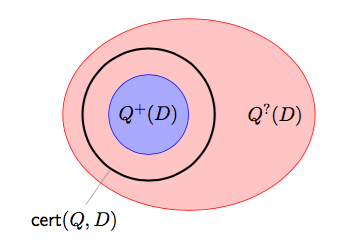
\includegraphics[scale=0.5]{set1}
\end{figure}


\begin{mylem}
	$$\sigma_\Sigma(cert_{\bot}((*,R,H,P),D)) \subseteq cert_{\bot}((\Sigma,R,H,P),D)$$ 
\end{mylem}
\begin{proof}
	\begin{align*}
		Q = (\Sigma,R,H,P) \\
		x \in^n \sigma_\Sigma(cert_{\bot}(Q_*,D)) & \Rightarrow \sum_{z \in \{y | y \in cert_{\bot}(Q_*,D) \land \sigma_\Sigma(y) = x \} }{cert_{\bot}(Q*,D)(z)} \geq n \\
		Moreover \\
		\forall g, cert_\bot(Q_*,D) &  \subseteq Eval(Q_*,g(D)) \\
		Then \\
		x \in^n \sigma_\Sigma(cert_{\bot}(Q_*,D)) & \Rightarrow \forall g , \sum_{z \in \{y | y \in Eval(Q_*,g(D)) \land \sigma_\Sigma(y) = x \} }{Eval(Q_*,g(D)) (z)} \geq n \\
		& \Rightarrow \forall g, Eval(Q,g(D))(x) \geq n \\
		& \Rightarrow x \in^n cert_\bot(Q,D) \\
	\end{align*}
\end{proof}	
\fi

\begin{figure}[H]
\caption{\label{q+} Translation $Q \rightarrow (Q^+,Q^?)$ }
\begin{mdframed}
	\fontsize{8}{6}
\begin{align*}
	(\Sigma,R,H,P)^+ & \rightarrow (\Sigma,R,H^*,P) \\
	(\Sigma,R,H,P)^? & \rightarrow (\Sigma,R,H^{**},P) 
\end{align*}
\end{mdframed}
\end{figure}

\begin{figure}[H]
	\caption{\label{h*} Translation $H \rightarrow H^*$ }
	\begin{mdframed}
		\fontsize{8}{6}
\begin{align*}
	(H_1 \land H_2)^* & \rightarrow H_1^* \land H_2^* \\
	(H_1 \lor H_2)^* & \rightarrow H_1^* \lor H_2^* \\
	(r_i.a_i = c_i)^* & \rightarrow r_i.a_i = c_i \\
	(r_i.a_i \neq c_i)^*& \rightarrow r_i.a_i \neq c_i \land const(r_i.a_i)\\
	(r_i.a_i > c_i)^*& \rightarrow r_i.a_i > c_i \\
	(r_i.a_i < c_i)^*& \rightarrow r_i.a_i < c_i \\
	(r_i.a_i = r_j.a_j)^* & \rightarrow r_i.a_i = r_j.a_j \\
	(r_i.a_i \neq r_j.a_j)^* & \rightarrow r_i.a_i \neq r_j.a_j \land const(r_i.a_i) \land const(r_j.a_j)\\
	(r_i.a_i > r_j.a_j)^* & \rightarrow r_i.a_i > r_j.a_j \\
	(r_i.a_i < r_j.a_j)^* & \rightarrow r_i.a_i < r_j.a_j \\
	(r_i.a_i = p_j)^* & \rightarrow r_i.a_i = p_j \\
	(r_i.a_i \neq p_j)^* & \rightarrow r_i.a_i \neq p_j \land const(r_i.a_i) \land const(p_j)\\
	(r_i.a_i > p_j)^* & \rightarrow r_i.a_i > p_j \\
	(r_i.a_i < p_j)^* & \rightarrow r_i.a_i < p_j \\
	exists(Q)^* & \rightarrow exists(Q^+) \\
	notexists(Q)^* & \rightarrow notexists(Q^?) \\
\end{align*}
\end{mdframed}
\end{figure}

\begin{figure}[H]
	\caption{\label{h**} Translation $H \rightarrow H^{**}$ }
		\begin{mdframed}
			\fontsize{8}{6}
\begin{align*}
	(H_1 \land H_2)^{**} & \rightarrow H_1^{**} \land H_2^{**} \\
	(H_1 \lor H_2)^{**} & \rightarrow H_1^{**} \lor H_2^{**} \\
	(r_i.a_i = c_i)^{**} & \rightarrow r_i.a_i = c_i \lor null(r_i.a_i)\\
	(r_i.a_i \neq c_i)^{**}& \rightarrow r_i.a_i \neq c_i \\
	(r_i.a_i > c_i)^{**} & \rightarrow r_i.a_i > c_i \lor null(r_i.a_i)\\
	(r_i.a_i < c_i)^{**} & \rightarrow r_i.a_i < c_i \lor null(r_i.a_i)\\
	(r_i.a_i = r_j.a_j)^{**} & \rightarrow r_i.a_i = r_j.a_j \lor null(r_i.a_i) \lor null(r_j.a_j)\\
	(r_i.a_i \neq r_j.a_j)^{**} & \rightarrow r_i.a_i \neq r_j.a_j \\
	(r_i.a_i > r_j.a_j)^{**} & \rightarrow r_i.a_i > r_j.a_j \lor \left( (null(r_i.a_i) \lor null(r_j.a_j)) \land r_i.a_i \neq r_j.a_j \right) \\
	(r_i.a_i < r_j.a_j)^{**} & \rightarrow r_i.a_i < r_j.a_j \lor \left( (null(r_i.a_i) \lor null(r_j.a_j)) \land r_i.a_i \neq r_j.a_j \right) \\
	(r_i.a_i = p_j)^{**} & \rightarrow r_i.a_i = p_j \lor null(r_i.a_i) \lor null(p_j)\\
	(r_i.a_i \neq p_j)^{**} & \rightarrow r_i.a_i \neq p_j \\
	(r_i.a_i > p_j)^{**} & \rightarrow r_i.a_i > p_j \lor \left( (null(r_i.a_i) \lor null(p_j)) \land r_i.a_i \neq p_j \right) \\
	(r_i.a_i < p_j)^{**} & \rightarrow r_i.a_i < p_j \lor \left( (null(r_i.a_i) \lor null(p_j)) \land r_i.a_i \neq p_j \right) \\
	exists(Q)^{**} & \rightarrow exists(Q^?) \\
	notexists(Q)^{**} & \rightarrow notexists(Q^+) \\
\end{align*}
	\end{mdframed}
\end{figure}

The key to understand this algorithm, is that $Q^?$ actually compute every answers that might be a certain answer. Indeed as soon as there exist a valuation such that $x \in Q(v(D))$ then $x \in Q^?(D)$. This property is ensure by the fact that the equality is replace with a disjunction checking if the attributes are nulls. As soon as one of the attribute is null then a valuation might exists which validate the equality. Conversely $Q^+$ ensure that difference are verify for every valuation, by replacing them with a conjunction ensuring that no nulls are involve. Then it's easy to understand that we can demonstrate that: if we assume that $Q^+$ evaluation only return certain answers, then $Q^?$ return at least all of them. And if we assume that $Q^?$ computes at least every certain answers, then $Q^+$ will only return certain answers.

\begin{mylem}
	$$\forall Q \in \llbracket SQL \rrbracket, \sigma_\Sigma(cert_{\bot}(Q_*,D)) = cert_{\bot}(Q,D)$$ 
\end{mylem}

\begin{proof}
	\begin{align*}
		Q = (\Sigma,R,H,P) \\
		x \in^n \sigma_\Sigma(cert_{\bot}(Q_*,D)) & \Rightarrow \sum_{z \in \{y | y \in cert_{\bot}(Q_*,D) \land \sigma_\Sigma(y) = x \} }{cert_{\bot}(Q*,D)(z)} \geq n \\
		Moreover \\
		\forall g, cert_\bot(Q_*,D) &  \subseteq Eval(Q_*,g(D)) \\
		Then \\
		x \in^n \sigma_\Sigma(cert_{\bot}(Q_*,D)) & \Rightarrow \forall g , \sum_{z \in \{y | y \in Eval(Q_*,g(D)) \land \sigma_\Sigma(y) = x \} }{Eval(Q_*,g(D)) (z)} \geq n \\
		& \Rightarrow \forall g, Eval(Q,g(D))(x) \geq n \\
		& \Rightarrow x \in^n cert_\bot(Q,D) \\
	\end{align*}
	\begin{align*}
		Q = (\Sigma,R,H,P) \\
		x \notin \sigma_\Sigma(cert_{\bot}(Q_*,D)) & \Rightarrow \sum_{z \in \{y | y \in cert_{\bot}(Q_*,D) \land \sigma_\Sigma(y) = x \} }{cert_{\bot}(Q_*,D)(z)} = 0 \\
		& \Rightarrow \forall y, \sigma_{\Sigma}(y) \neq x  \lor cert_{\bot}(Q_*,D)(y) = 0 \\
		& \Rightarrow \forall y, \sigma_{\Sigma}(y) \neq x  \lor \exists v, v(y) \notin Eval_{SQL}(Q_*,v(D)) \\
		& \Rightarrow \exists v, v(x) \notin \sigma_{\Sigma}(Eval_{SQL}(Q_*,v(D))) \\
		& \Rightarrow \exists v, v(x) \notin Eval_{SQL}(Q,D) \\
		& \Rightarrow x \notin cert_\bot(Q,D) \\
	\end{align*}
\end{proof}

\begin{myprop}
	\label{prop2}
	$$\forall Q \in \llbracket SQL \rrbracket, Eval_{SQL}(Q^+,D) \subseteq cert_\bot(Q,D)$$
\end{myprop}
\begin{myprop}
	\label{prop3}
	$$\forall Q \in \llbracket SQL \rrbracket, cert_\bot(Q,D) \subseteq Eval_{SQL}(Q^?,D)$$
\end{myprop}


\begin{proof}
	The proof of (2) is made by induction over the query $Q$ assuming only (3).
	\\We only detail critical case a more complete proof can be found in appendix.
	\iffalse
	\begin{align*}
		Q = (\Sigma,R,r_i.a_i \neq p_i,P) \\
		x \in^n Eval_{SQL}(Q^+,D) & \Rightarrow \sum_{z \in \{y | y \in Eval_{SQL}(Q_*^+,D) \land \sigma_\Sigma(y) = x \} }{Eval_{SQL}(Q_*^+,D)(z)} \geq n  \\
		Moreover\\
		Eval_{SQL}(Q^+_*,D)(z)  \geq k & \Rightarrow  Eval_{SQL}((*,R,(r_i.a_i \neq p_i )^*,P),D)(z) \geq k \\
		& \Rightarrow Eval_{SQL}((*,R,r_i.a_i \neq p_i \land const(r_i,a_i) \land const(p_i),P),D)(z)  \geq k \\
		& \Rightarrow R^\times(x) \geq k \land x[r_i.a_i] \neq P[p_i] \land \forall t, x[r_i.a_i] \neq \bot_t \land \forall t, P[p_i] \neq \bot_t \\
		Moreover \\
		\forall t, x[r_i.a_i] \neq \bot_t \land \forall t, P[p_i] \neq \bot_t & \Rightarrow \forall h, h(x)[r_i.a_i] = x[r_i.a_i] \land h(P)[p_i] = P[p_i] \\
		Then \\
		Eval_{SQL}(Q^+_*,D)(z)  \geq k & \Rightarrow R^\times(x) \gek k \land \forall h, h(x)[r_i.a_i] \neq h(P)[p_i] \\
		& \Rightarrow cert_\bot(Q_*,D)(z) = k \\
		Then \\
		x \in^n Eval_{SQL}(Q^+,D) & \Rightarrow \sum_{z \in \{y | y \in Eval_{SQL}(Q_*^+,D) \land \sigma_\Sigma(y) = x \} }{cert_\bot(Q_*,D)(z)} \geq n  \\
		& \Rightarrow x \in^n cert_\bot(Q,D) \\
	\end{align*}
	\fi
	\begin{align*}
		Q = (\Sigma,R,notexists(Q'),P) \\
		x \in^n Eval_{SQL}(Q^+,D) & \Rightarrow \sum_{z \in \{y | y \in Eval_{SQL}(Q_*^+,D) \land \sigma_\Sigma(y) = x \} }{Eval_{SQL}(Q_*^+,D)(z)} \geq n  \\
		Moreover\\
		Eval_{SQL}(Q^+_*,D)(z)  \geq k & \Rightarrow  Eval_{SQL}((*,R,notexists(Q')^*,P),D)(z)  \geq k \\
		& \Rightarrow  Eval_{SQL}((*,R,notexists(Q'^?),P),D)(z)  \geq k \\
		& \Rightarrow R^\times(z) \geq k \land Eval_{SQL}(Q'[z]^?,D) = \emptyset \\
		& \Rightarrow R^\times(z) \geq k \land cert_\bot(Q'[z],D) = \emptyset \\
		& \Rightarrow R^\times(z) \geq k \land \forall h, \forall w, h(w) \notin Eval_{SQL}(Q'[h(z)],h(D)) \\
		& \Rightarrow R^\times(z) \geq k \land \forall h , Eval_{SQL}(Q'[h(z)],h(D)) = \emptyset \\
		& \Rightarrow R^\times(z) \geq k \land \forall h, h(z) \in Eval_{SQL}((*,R,notexists(Q'),h(P)),h(D)) \\
		& \Rightarrow cert_\bot(Q_*,D)(z) \geq k \\
		Then \\
		x \in^n Eval_{SQL}(Q^+,D) & \Rightarrow \sum_{z \in \{y | y \in Eval_{SQL}(Q_*^+,D) \land \sigma_\Sigma(y) = x \} }{cert_\bot(Q_*,D)(z)} \geq n  \\
		& \Rightarrow x \in^n cert_\bot(Q,D) \\
	\end{align*}
\end{proof}

\begin{proof}
	The proof of (3) is made by induction over the query $Q$ assuming only (2).
	\\We only detail critical case a more complete proof can be found in appendix.
	\iffalse
	\begin{align*}
		Q = (\Sigma,R,r_i.a_i = r_j.a_j,P) \\
		x \in^n cert_\bot(Q,D) & \Rightarrow \sum_{z \in \{y | y \in cert_\bot(Q_*,D) \land \sigma_\Sigma(y) = x \} }{cert_\bot(Q_*,D)(z)} \geq n \\
		Moreover\\
		cert_\bot(Q_*,D)(z)  \geq k & \Rightarrow  \forall h, h(z) \in^k Eval_{SQL}(Q_*,h(D)) \\
		& \Rightarrow  \forall h,\forall t, R^\times(z) \geq k \land h(z)[r_i.a_i] = h(z)[r_j.a_j] \land h(z)[r_i.a_i] \neq \bot_t \land h(z)[r_j.a_j] \neq \bot_t  \\
		Moreover \\
		\mbox{ TRUE} & \Rightarrow \forall g,\forall t, g(z)[r_i.a_i] \neq \bot_t \\
		\forall h, h(z)[r_i.a_i] = h(z)[r_j.a_j] & \Rightarrow \exists h, h(z)[r_i.a_i] = h(z)[r_j.a_j] \\
		 & \Rightarrow z[r_i.a_i] = z[r_j.a_j] \lor (\exists t, z[r_i.a_i]  = \bot_t) \lor (\exists t, z[r_j.a_j] = \bot_t) \\
		Then\\
		cert_\bot(Q_*,D)(z)  \geq k & \Rightarrow  R^\times(z) \geq k \land z[r_i.a_i] = z[r_j.a_j] \lor (\exists t, z[r_i.a_i]  = \bot_t) \lor (\exists t, z[r_j.a_j] = \bot_t) \\
		& \Rightarrow R^\times(z) \geq k \land z \in Eval_{SQL}((*,R,(r_i.a_i = r_j.a_j \lor null(r_i.a_i) \lor null(r_j.a_j)),P),D) \\
		& \Rightarrow R^\times(z) \geq k \land z \in Eval_{SQL}((*,R,(r_i.a_i = r_j.a_j)^{**},P),D) \\
		& \Rightarrow Eval_{SQL}((*,R,r_i.a_i = r_j.a_j,P)^?,D)(z) \geq k \\
		Then \\
		x \in^n cert_\bot(Q,D) &\Rightarrow  \sum_{z \in \{y | y \in cert_\bot(Q_*,D) \land \sigma_\Sigma(y) = x \} }{Eval_{SQL}(Q_*^?,D)(z)} \geq n \\
		& \Rightarrow x \in^n Eval_{SQL}(Q^?,D) \\
	\end{align*}
	\fi
	\begin{align*}
		Q = (\Sigma,R,notexists(Q'),P) \\
		x \in^n cert_\bot(Q,D) & \Rightarrow \sum_{z \in \{y | y \in cert_\bot(Q_*,D) \land \sigma_\Sigma(y) = x \} }{cert_\bot(Q_*,D)(z)} \geq n \\
		Moreover\\
		cert_\bot(Q_*,D)(z)  \geq k  & \Rightarrow  R^\times(z) \geq k \land \forall h, h(z) \in  Eval_{SQL}((*,R,notexists(Q'),h(P)),h(D)) \\
		& \Rightarrow  R^\times(z) \geq k \land  \forall h, Eval_{SQL}(Q'[h(z)],h(D)) = \emptyset \\
		&  \Rightarrow  R^\times(z) \geq k \land  cert_\bot(Q'[z],D) = \emptyset \\
		&  \Rightarrow  R^\times(z) \geq k \land  Eval(Q'[z]^+,D) = \emptyset \\
		&  \Rightarrow  R^\times(z) \geq k \land z \in Eval_{SQL}((*,R,notexists(Q'^+),P),D) \\
		&  \Rightarrow  R^\times(z) \geq k \land z \in Eval_{SQL}((*,R,notexists(Q')^{**},P),D) \\
		&  \Rightarrow  Eval_{SQL}((*,R,notexists(Q'),P)^?,D)(z) \geq k \\
		Then \\
		x \in^n cert_\bot(Q,D) &\Rightarrow  \sum_{z \in \{y | y \in posi_\bot(Q_*,D) \land \sigma_\Sigma(y) = x \} }{Eval_{SQL}(Q_*^?,D)(z)} \geq n \\
		& \Rightarrow x \in^n Eval_{SQL}(Q^?,D) \\
	\end{align*}
\end{proof}

\iffalse
\begin{proof}
	Assume (5).
	\\By induction :
	\begin{align*}
		Q = (\Sigma,R,H_1\land H_2,P) \\
		x \in^n Eval_{SQL}(Q^+,D) & \Rightarrow \sum_{z \in \{y | y \in Eval_{SQL}(Q_*^+,D) \land \sigma_\Sigma(y) = x \} }{Eval_{SQL}(Q_*^+,D)(z)} \geq n  \\
		Moreover\\
		Eval_{SQL}(Q^+_*,D)(z)  = k & \Rightarrow  Eval_{SQL}((*,R,H_1^*\land H_2^*,P),D)(z)  = k \\
		& \Rightarrow  (Eval_{SQL}((*,R,H_1^*,P),D) \cap Eval_{SQL}((*,R,H_2^*,P),D))(z)  = k \\
		& \Rightarrow  (Eval_{SQL}((*,R,H_1,P)^+,D) \cap Eval_{SQL}((*,R,H_2,P)^+,D))(z)  = k \\
		& \Rightarrow  (Eval_{SQL}((*,R,H_1,P)^+,D))(x) \geq k \land  (Eval_{SQL}((*,R,H_2,P)^+,D))(z)  \geq k \\
		& \Rightarrow  (cert_\bot((*,R,H_1,P),D))(x) \geq k \land  (cert_\bot((*,R,H_2,P),D))(z)  \geq k \\
		& \Rightarrow  (cert_\bot((*,R,H_1,P),D) \cap cert_\bot((*,R,H_2,P),D))(z)  \geq k \\
		& \Rightarrow  (cert_\bot((*,R,H_1 \land H_2,P),D))(z)  \geq k \\
		& \Rightarrow  (cert_\bot(Q_*,D))(z)  \geq k \\
		Then \\
		x \in^n Eval_{SQL}(Q^+,D) & \Rightarrow \sum_{z \in \{y | y \in Eval_{SQL}(Q_*^+,D) \land \sigma_\Sigma(y) = x \} }{cert_\bot(Q_*,D)(z)} \geq n  \\
		& \Rightarrow x \in^n cert_\bot(Q,D) \\
	\end{align*}
	\begin{align*}
		Q = (\Sigma,R,H_1\lor H_2,P) \\
		x \in^n Eval_{SQL}(Q^+,D) & \Rightarrow \sum_{z \in \{y | y \in Eval_{SQL}(Q_*^+,D) \land \sigma_\Sigma(y) = x \} }{Eval_{SQL}(Q_*^+,D)(z)} \geq n  \\
		Moreover\\
		Eval_{SQL}(Q^+_*,D)(z)  = k & \Rightarrow  Eval_{SQL}((*,R,H_1^*\lor H_2^*,P),D)(z)  = k \\
		& \Rightarrow  (Eval_{SQL}((*,R,H_1^*,P),D) \cup Eval_{SQL}((*,R,H_2^*,P),D))(z)  = k \\
		& \Rightarrow  (Eval_{SQL}((*,R,H_1,P)^+,D) \cup Eval_{SQL}((*,R,H_2,P)^+,D))(z)  = k \\
		& \Rightarrow  (Eval_{SQL}((*,R,H_1,P)^+,D))(x) \geq k \lor  (Eval_{SQL}((*,R,H_2,P)^+,D))(z)  \geq k \\
		& \Rightarrow  (cert_\bot((*,R,H_1,P),D))(x) \geq k \lor  (cert_\bot((*,R,H_2,P),D))(z)  \geq k \\
		& \Rightarrow  (cert_\bot((*,R,H_1,P),D) \cup cert_\bot((*,R,H_2,P),D))(z)  \geq k \\
		& \Rightarrow  (cert_\bot((*,R,H_1 \lor H_2,P),D))(z)  \geq k \\
		& \Rightarrow  (cert_\bot(Q_*,D))(z)  \geq k \\
		Then \\
		x \in^n Eval_{SQL}(Q^+,D) & \Rightarrow \sum_{z \in \{y | y \in Eval_{SQL}(Q_*^+,D) \land \sigma_\Sigma(y) = x \} }{cert_\bot(Q_*,D)(z)} \geq n  \\
		& \Rightarrow x \in^n cert_\bot(Q,D) \\
	\end{align*}
	\begin{align*}
		Q = (\Sigma,R,notexists(Q'),P) \\
		x \in^n Eval_{SQL}(Q^+,D) & \Rightarrow \sum_{z \in \{y | y \in Eval_{SQL}(Q_*^+,D) \land \sigma_\Sigma(y) = x \} }{Eval_{SQL}(Q_*^+,D)(z)} \geq n  \\
		Moreover\\
		Eval_{SQL}(Q^+_*,D)(z)  = k & \Rightarrow  Eval_{SQL}((*,R,notexists(Q')^*,P),D)(z)  = k \\
		& \Rightarrow  Eval_{SQL}((*,R,notexists(Q'^?),P),D)(z)  = k \\
		& \Rightarrow R(z) = k \land Eval_{SQL}(Q'[z]^?,D) = \emptyset \\
		& \Rightarrow R(z) = k \land cert_\bot(Q'[z],D) = \emptyset \\
		& \Rightarrow R(z) = k \land \forall h, \forall w, h(w) \notin Eval_{SQL}(Q'[h(z)],h(D)) \\
		& \Rightarrow R(z) = k \land \forall h , Eval_{SQL}(Q'[h(z)],h(D)) = \emptyset \\
		& \Rightarrow R(z) = k \land \forall h, h(z) \in Eval_{SQL}((*,R,notexists(Q'),h(P)),h(D)) \\
		& \Rightarrow cert_\bot(Q_*,D)(z) = k \\
		Then \\
		x \in^n Eval_{SQL}(Q^+,D) & \Rightarrow \sum_{z \in \{y | y \in Eval_{SQL}(Q_*^+,D) \land \sigma_\Sigma(y) = x \} }{cert_\bot(Q_*,D)(z)} \geq n  \\
		& \Rightarrow x \in^n cert_\bot(Q,D) \\
	\end{align*}
	\begin{align*}
		Q = (\Sigma,R,r_i.a_i \neq p_i,P) \\
		x \in^n Eval_{SQL}(Q^+,D) & \Rightarrow \sum_{z \in \{y | y \in Eval_{SQL}(Q_*^+,D) \land \sigma_\Sigma(y) = x \} }{Eval_{SQL}(Q_*^+,D)(z)} \geq n  \\
		Moreover\\
		Eval_{SQL}(Q^+_*,D)(z)  = k & \Rightarrow  Eval_{SQL}((*,R,(r_i.a_i \neq p_i )^*,P),D)(z)  = k \\
		& \Rightarrow Eval_{SQL}((*,R,r_i.a_i \neq p_i \land const(r_i,a_i) \land const(p_i),P),D)(z)  = k \\
		& \Rightarrow R(x) = k \land x[r_i.a_i] \neq P[p_i] \land \forall t, x[r_i.a_i] \neq \bot_t \land \forall t, P[p_i] \neq \bot_t \\
		Moreover \\
		\forall t, x[r_i.a_i] \neq \bot_t \land \forall t, P[p_i] \neq \bot_t & \Rightarrow \forall h, h(x)[r_i.a_i] = x[r_i.a_i] \land h(P)[p_i] = P[p_i] \\
		Then \\
		Eval_{SQL}(Q^+_*,D)(z)  = k & \Rightarrow R(x) = k \land \forall h, h(x)[r_i.a_i] \neq h(P)[p_i] \\
		& \Rightarrow cert_\bot(Q_*,D)(z) = k \\
		Then \\
		x \in^n Eval_{SQL}(Q^+,D) & \Rightarrow \sum_{z \in \{y | y \in Eval_{SQL}(Q_*^+,D) \land \sigma_\Sigma(y) = x \} }{cert_\bot(Q_*,D)(z)} \geq n  \\
		& \Rightarrow x \in^n cert_\bot(Q,D) \\
	\end{align*}
\end{proof}

\begin{proof}
	Assume (4).
	\\By induction ...
	\begin{align*}
		Q = (\Sigma,R,H_1\land H_2,P) \\
		x \in^n cert_\bot(Q,D) & \Rightarrow \sum_{z \in \{y | y \in posi_\bot(Q_*,D) \land \sigma_\Sigma(y) = x \} }{cert_\bot(Q_*,D)(z)} \geq n \\
		Moreover\\
		cert_\bot(Q_*,D)(z)  = k & \Rightarrow R(z) = k \land \exists h, h(z) \in Eval_{SQL}((*,R,H_1\land H_2,h(P)),h(D)) \\
		& \Rightarrow R(z) = k \land \exists h, h(z) \in Eval_{SQL}((*,R,H_1,h(P)),h(D)) \land h(z) \in Eval_{SQL}((*,R,H_1,h(P)),h(D))\\
		& \Rightarrow cert_\bot((*,R,H_1,P),D)(z) \geq k \land  cert_\bot((*,R,H_2,P),D)(z) \geq k\\
		&\Rightarrow Eval_{SQL}((*,R,H_1,P)^?,D)(z) \geq k \land  Eval_{SQL}((*,R,H_2,P)^?,D)(z) \geq k\\
		&\Rightarrow Eval_{SQL}((*,R,H_1^{**},P),D)(z) \geq k \land  Eval_{SQL}((*,R,H_2^{**},P),D)(z) \geq k\\
		&\Rightarrow Eval_{SQL}((*,R,H_1^{**} \land H_2^{**},P),D)(z) \geq k\\
		&\Rightarrow Eval_{SQL}((*,R,H_1 \land H_2,P)^?,D)(z) \geq k\\
		&\Rightarrow Eval_{SQL}(Q_*^?,D)(z) \geq k\\
		Then \\
		x \in^n cert_\bot(Q,D) &\Rightarrow  \sum_{z \in \{y | y \in posi_\bot(Q_*,D) \land \sigma_\Sigma(y) = x \} }{Eval_{SQL}(Q_*^?,D)(z)} \geq n \\
		& \Rightarrow x \in^n Eval_{SQL}(Q^?,D) \\
	\end{align*}
	
	\begin{align*}
		Q = (\Sigma,R,notexists(Q'),P) \\
		x \in^n cert_\bot(Q,D) & \Rightarrow \sum_{z \in \{y | y \in posi_\bot(Q_*,D) \land \sigma_\Sigma(y) = x \} }{cert_\bot(Q_*,D)(z)} \geq n \\
		Moreover\\
		cert_\bot(Q_*,D)(z)  = k  & \Rightarrow  R(z) = k \land \exists h, h(z) \in  Eval_{SQL}((*,R,notexists(Q'),h(P)),h(D)) \\
		& \Rightarrow  R(z) = k \land  \exists h, Eval_{SQL}(Q'[h(z)],h(D)) = \emptyset \\
		&  \Rightarrow  R(z) = k \land  \llbracket w^n| \forall g, g(w) \in^n Eval_{SQL}((Q'[g(z)]),g(D)) \rrbracket = \emptyset \\ 
		&  \Rightarrow  R(z) = k \land  cert_\bot(Q'[z],D) = \emptyset \\
		&  \Rightarrow  R(z) = k \land  Eval(Q'[z]^+,D) = \emptyset \\
		&  \Rightarrow  R(z) = k \land z \in Eval_{SQL}((*,R,notexists(Q'^+),P),D) \\
		&  \Rightarrow  R(z) = k \land z \in Eval_{SQL}((*,R,notexists(Q')^{**},P),D) \\
		&  \Rightarrow  Eval_{SQL}((*,R,notexists(Q'),P)^?,D)(z) = k \\
		Then \\
		x \in^n cert_\bot(Q,D) &\Rightarrow  \sum_{z \in \{y | y \in posi_\bot(Q_*,D) \land \sigma_\Sigma(y) = x \} }{Eval_{SQL}(Q_*^?,D)(z)} \geq n \\
		& \Rightarrow x \in^n Eval_{SQL}(Q^?,D) \\
	\end{align*}
	
	\begin{align*}
		Q = (\Sigma,R,r_i.a_i = r_j.a_j,P) \\
		x \in^n cert_\bot(Q,D) & \Rightarrow \sum_{z \in \{y | y \in posi_\bot(Q_*,D) \land \sigma_\Sigma(y) = x \} }{cert_\bot(Q_*,D)(z)} \geq n \\
		Moreover\\
		cert_\bot(Q_*,D)(z)  = k & \Rightarrow  R(z) = k \land \exists h, h(z) \in Eval_{SQL}((*,R,r_i.a_i = r_j.a_j,h(P)),h(D)) \\
		& \Rightarrow  R(z) = k \land  \exists h, h(z)[r_i.a_i] = h(z)[r_j.a_j] \land h(z)[r_i.a_i] \neq \bot \land h(z)[r_j.a_j] \neq \bot  \\
		Moreover \\
		\exists h, h(z)[r_i.a_i] = h(z)[r_j.a_j] & \Rightarrow z[r_i.a_i] = z[r_j.a_j] \lor z[r_i.a_i]  = \bot \lor z[r_j.a_j] = \bot \\
		\forall g, g(z)[r_i.a_i] \neq \bot & \Rightarrow \mbox{ TRUE} \\
		Then\\
		cert_\bot(Q_*,D)(z)  = k & \Rightarrow  R(z) = k \land z[r_i.a_i] = z[r_j.a_j] \lor z[r_i.a_i]  = \bot \lor z[r_j.a_j] = \bot \\
		& \Rightarrow R(z) =k \land z \in Eval_{SQL}((*,R,(r_i.a_i = r_j.a_j \lor null(r_i.a_i) \lor null(r_j.a_j)),P),D) \\
		& \Rightarrow R(z) =k \land z \in Eval_{SQL}((*,R,(r_i.a_i = r_j.a_j)^{**},P),D) \\
		& \Rightarrow Eval_{SQL}((*,R,r_i.a_i = r_j.a_j,P)^?,D)(z) = k \\
		Then \\
		x \in^n cert_\bot(Q,D) &\Rightarrow  \sum_{z \in \{y | y \in posi_\bot(Q_*,D) \land \sigma_\Sigma(y) = x \} }{Eval_{SQL}(Q_*^?,D)(z)} \geq n \\
		& \Rightarrow x \in^n Eval_{SQL}(Q^?,D) \\
	\end{align*}
\end{proof}

\fi

We have proven that the evaluation algorithm such that we translate a query $Q$ in $Q^+$ and then evaluate $Q^+$ with standard SQL semantics has \emph{correctness guarantee}. Indeed we have even proven that such translation is valid as long as $Q^+$ computes a subset of certain answers and $Q^?$ computes at least all of them. It's easy to understand that work may be done in order to improve the over approximation of the certain answers without any loose.